\documentclass[a4paper,12pt,twoside]{article}

\usepackage{../IyA.estilo.2015}
\usepackage{acronym}
\usepackage{caption}

%-------------------para incluir archivos graficos .gif------%
\epstopdfDeclareGraphicsRule{.gif}{png}{.png}{%
  convert gif:#1 png:\OutputFile
}
\AppendGraphicsExtensions{.gif}



%------------------Define box and box title style
\tikzstyle{mybox} = [draw=red, fill=yellow!20, very thick,
    rectangle, rounded corners, inner sep=10pt, inner ysep=20pt]
\tikzstyle{fancytitle} =[fill=blue!80, text=white]

\tikzstyle{grupos} = [draw=blue, fill=green!20, very thick,
    rectangle, rounded corners, inner sep=10pt, inner ysep=20pt]
\tikzstyle{fancytitle.grupos} =[fill=blue, text=white, ellipse]


\newcommand{\fullref}[1]{\ref{#1} de la p\'agina \pageref{#1}}

%-------------------------------------Encabezado
\fancyhead[RO,LE]{\small{{\bf \large Instrumentos y Avi\'onica} \\
\textcolor{blue}{\bf Medidores de datos de aire}\\
P\'agina \thepage \ de \pageref{LastPage}
                 }
                 }

\fancyhead[RE,LO]{
	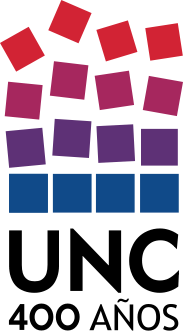
\includegraphics[height=1.5cm]{imagenes/logos/400-anios.png}
	
\includegraphics[height=1.2cm]{imagenes/logos/logoUNC.png}
	
\includegraphics[height=1.2cm]{imagenes/logos/fcefyn.png}
	
\includegraphics[height=1.2cm]{imagenes/logos/dpto-aero-logo.png}
}

%----------------------------------Caratula
\title{Medidores de datos de aire}
\author{Ing. Jorge Garcia (jgarcia@efn.uncor.edu)}
\date{\today}

\begin{document}

\renewcommand{\tablename}{Tabla}

\newcommand{\ESPACIO}{\rule{0in}{3ex}}

\thispagestyle{fancy}
\maketitle

\thispagestyle{fancy}
\tableofcontents

% Circuitos de presiones estática y total. Toma de presiones alternativas
% Altímetros barométricos, servoaltímetros. Codificadores de altura
% Vari\'ometros
% Velocímetros. Machmetros.
% Computadores centrales de datos de aire, su funci\'on

\newpage

\section{Circuitos de presiones estática y total. Toma de presiones alternativas}
\label{sec:Circuitos.de.presiones}

Un circuito de presiones pitot-estática consiste en un sistema de sensores e instrumentos sensibles 
a la presi\'on, que se utiliza en aeron\'autica para determinar 
la velocidad de una aeronave con relaci\'on al aire, la altitud y la variaci\'on de altitud. 
Los instrumentos que los utilizan son el Alt\'imetro, el Veloc\'imetro, el Vari\'ometro y, 
en algunos casos, el Indicador de N\'umero de Mach.

Otros instrumentos que pueden estar conectados al sistema son Computadores Centrales de Datos de Aire, 
registradores de datos de vuelo, controles de presurizacion de cabina, etc.

Los errores que pueden producirse en el sistema de pitot-est\'atica son extremadamente peligrosos.
Varios desastres de vuelos comerciales han tenido origen en fallos de este sistema. 

\begin{minipage}[m]{0.15\textwidth}
\href{https://www.youtube.com/watch?v=U8YaBYO9oj0}{
\includegraphics[width=\linewidth]{imagenes/iconos/video.jpg}}
%https://www.youtube.com/watch?v=U8YaBYO9oj0
\end{minipage}
\begin{minipage}[m]{0.80\textwidth}
  Ver por ejemplo el caso del vuelo 603 de Aero Perú el 2 de Octubre
  de 1996.
\end{minipage}


\begin{figure}[!h]
  \centering
  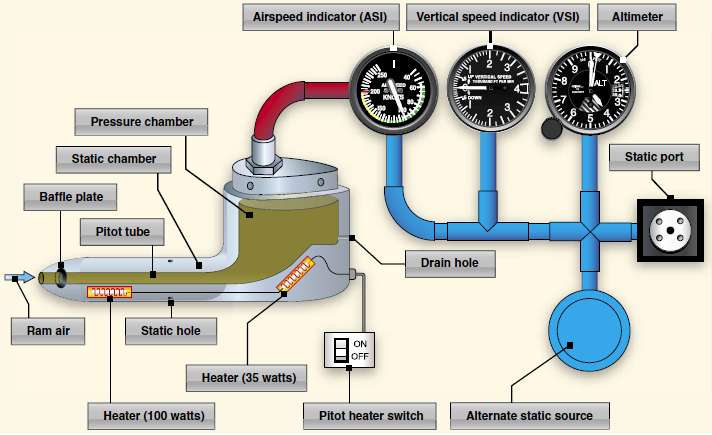
\includegraphics[width=\textwidth]{imagenes/Pitot-Static-System.png}
    \caption{Sistema de presi\'on  pitot-est\'atica t\'ipico. Gentileza Federal Aviation Administration}
\label{fig:sistema.pitot.estatica}
\end{figure}

\begin{figure}[!h]
  \centering
  \subfigure[Toma presi\'on pitot]{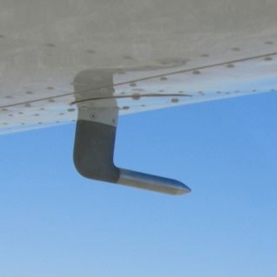
\includegraphics[width=0.4\textwidth]{imagenes/pitot_tube.jpg}}
  \subfigure[Ubicaci\'on tomas presi\'on pitot]{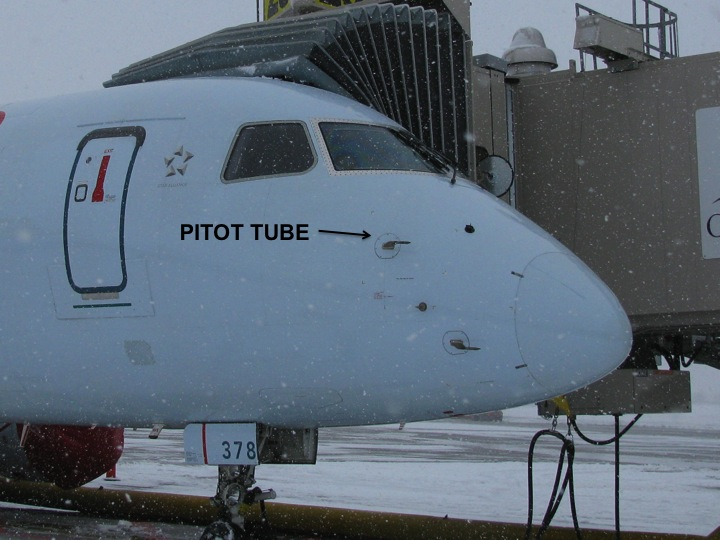
\includegraphics[width=0.4\textwidth]{imagenes/pitot_tube_ubicacion.jpg}}
  \caption{Tomas de presi\'on}
  \label{fig:tomas.presion}
\end{figure}

\begin{figure}[!h]
  \centering
  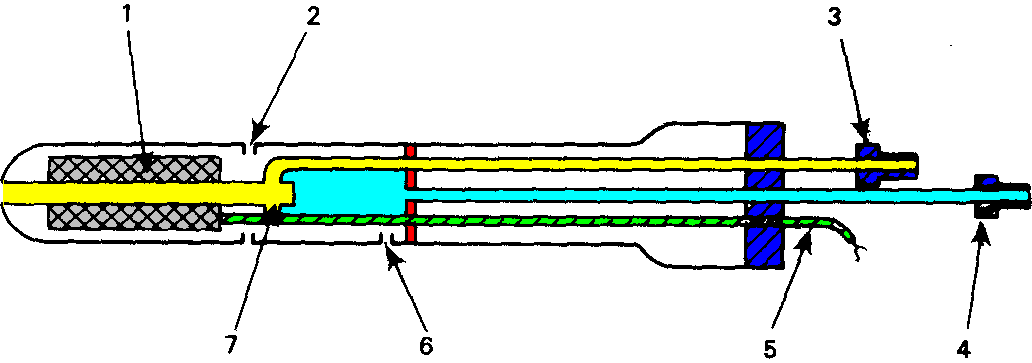
\includegraphics[width=\textwidth]{imagenes/basic_pitot_static_probe.png} 
 \captionsetup{singlelinecheck=off}
  \caption{Detalle constructivo de una sonda de presi\'on pitot y est\'atica.
{\footnotesize    \begin{multicols}{3}
    \begin{enumerate}
    \item Elemento calefactor
    \item Tomas est\'aticas
    \item Conexiones presi\'on pitot
    \item Conexiones presi\'on est\'atica
    \item Conexi\'on el\'ectrica elemento calefactor
    \item Drenaje
    \item Drenaje presi\'on pitot
    \end{enumerate}
  \end{multicols}
}
}
  \label{fig:pitot-static.probe}
\end{figure}


\begin{figure}[!htb]
  \centering
  \subfigure[Tomas de presi\'on est\'atica sobre el avi\'on]{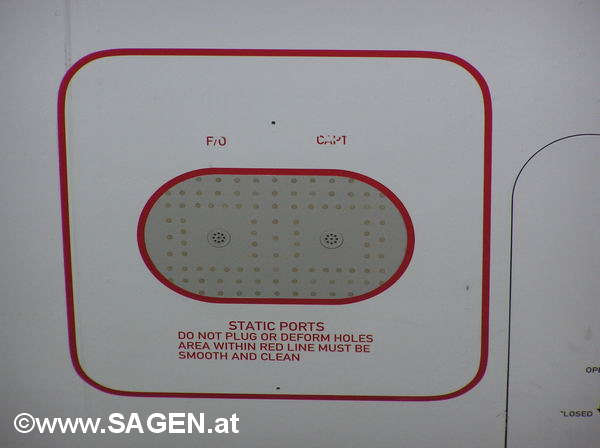
\includegraphics[width=0.4\textwidth]{imagenes/StaticPort.JPG}}
  \subfigure[Toma de presi\'on est\'atica avi\'on Convair F-102A]{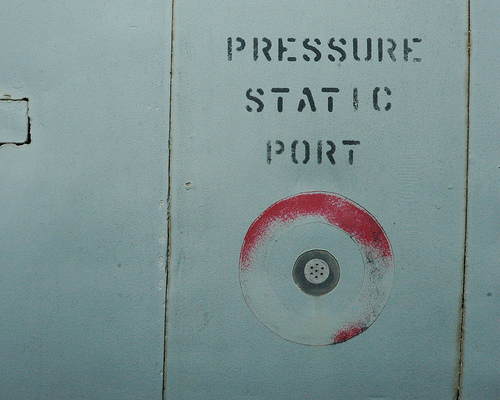
\includegraphics[width=0.4\textwidth]{imagenes/Convair_F-102A_Pressure_Static_Port.jpg}}

  \subfigure[Errores en la ubicaci\'on de las tomas de presi\'on est\'atica sobre el avi\'on.  Gentileza NASA]{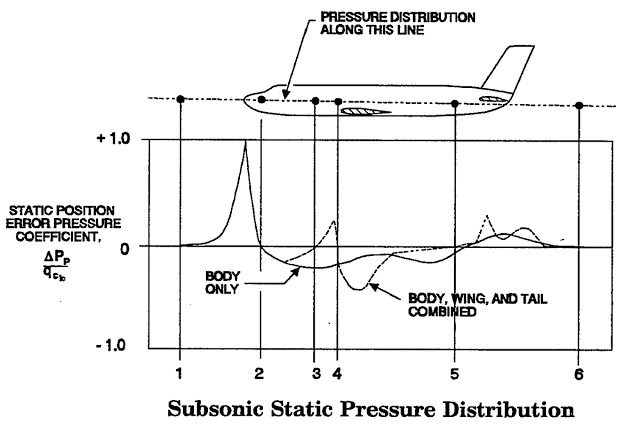
\includegraphics[width=0.94\textwidth]{imagenes/presion_estatica_sobre_avion.png}}
  \caption{Tomas de presi\'on est\'atica}
  \label{fig:tomas.presion.estatica}
\end{figure}




% \subsection{Accidentes a\'ereos con sospecha de haber sido provocados por problemas en sistema pitot-est\'atica}
% \label{sec:accidentes.aereos.problemas.pitot.estatica}

% \begin{itemize}
% \item 1 de noviembre de 1974, Northwest Airlines Flight 6231
% \item 6 de febrero de 1996, Birgenair Flight 301 
% \item 2 de octubre de 1996, Aeroperú Flight 603
% \item 10 de octubre de 1997, Austral Líneas Aéreas Flight 2553, \url{http://www.jiaac.gov.ar/boletin29.htm}
% \item 23 de febrero de 2008, base a\'erea de Guam, bombardero B-2
% \item 1 de junio de 2009, Air France Flight 447
% \end{itemize}

Para mayor informaci\'on sobre las mediciones de presi\'on est\'atica sobre la aeronave consultar:

\href{run:biblio/naca-rm-l57a09.pdf}{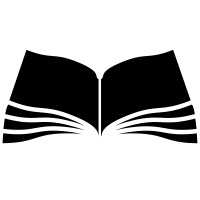
\includegraphics[width=0.1\textwidth]{imagenes/iconos/libro.png}}
\hspace{3mm}
\href{http://naca.central.cranfield.ac.uk/reports/1957/naca-rm-l57a09.pdf}{
\includegraphics[width=0.15\textwidth]{imagenes/iconos/www-logo.png}}
NACA-RM-L57A09 
Measurement of static pressure on aircraft



\newpage

\section{Alt\'imetro}
\label{altimetro}

El altímetro es un instrumento que se utiliza para
determinar la distancia vertical desde la aeronave hasta un determinado plano de
referencia. Forma parte de los instrumentos denominados Pitot-Estática.
Fu\'e inventado en 1928 por Paul Kollman, un ingeniero alem\'an emigrado a
Estados Unidos. Se populariz\'o luego de su uso por James Harold ``Jimmy'' Doolittle
durante el primer vuelo a ciegas utilizando instrumentos el 24 de setiembre de 1929.

\begin{figure}[!h]
  \centering
  \subfigure[Publicidad de \mbox{Kollsman}]{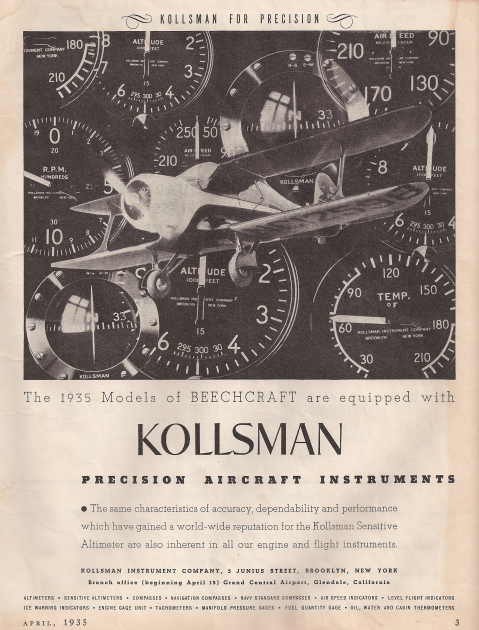
\includegraphics[width=0.43\textwidth]{imagenes/kollsman_publicidad.png}}
  \subfigure[Paul Kollsman]{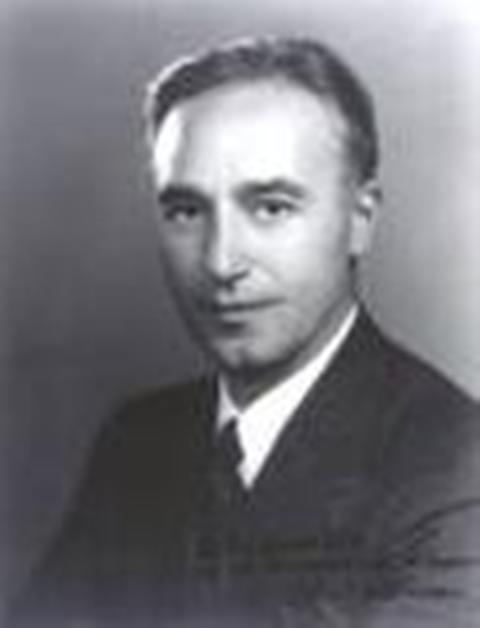
\includegraphics[width=0.43\textwidth]{imagenes/paul_kollsman.jpg}}

  \subfigure[Tablero instrumentos. Primer vuelo a ciegas]{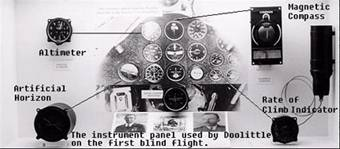
\includegraphics[width=0.95\textwidth]{imagenes/doolittle_instrumentos.jpg}}
  \caption{Primeros alt\'imetros}
  \label{fig:kollsman}
\end{figure}

El altímetro es uno de los instrumentos más importantes de una aeronave, 
ya que conociendo su funcionamiento, sus errores y la
forma correcta de reglarlo e interpretarlo, proporciona al piloto una
fehaciente informaci\'on relacionada con la distancia
vertical sobre obstáculos y lo ayuda a mantener una
separaci\'on reglamentaria con otras aeronaves, en cumplimiento de los rígidos
procedimientos de control de tránsito aéreo.

Igualmente, este instrumento se encuentra instalado en la torre de control y se utiliza para
suministrar al piloto, la lectura del instrumento que ha sido calibrado a la elevaci\'on del
aer\'odromo, para determinar la altitud de la aeronave con respecto a la estaci\'on para las
maniobras de despegue y aterrizaje, ya que durante estas fases del vuelo los pilotos tienen
necesidad de conocer la distancia vertical que los separa del terreno.

Los datos que se les comunican a los pilotos son las presiones locales (normalmente QNH \'o
QFE), las cuales introducirán en la sub-escala de su altímetro, para obtener indicaciones
de altitud o altura.

En las autorizaciones de aproximaci\'on y entrada en el circuito de tránsito se suministra el
reglaje altimétrico QNH. En aquellos países que se utiliza el reglaje QFE éste se identifica
claramente con objeto que no sea confundido con otro reglaje.

La utilizaci\'on de ajuste QNH o QFE, varía de unos países a otros. Inicialmente se utiliz\'o el
QFE, observándose luego, que debido a las limitaciones de los altímetros, entonces en su
uso, en aer\'odromos situados en lugares elevados, el ajuste QNH ofrecía indicaciones
altimétricas más útiles, tanto para los fines de margen vertical sobre el terreno, como para
los de separaci\'on vertical. %En Colombia el ajuste normalmente utilizado, es el QNH.

\textcolor{blue}{{\bf Isobaras:} líneas imaginarias que unen puntos de igual presi\'on atmosférica.}

Si las Isobaras se comportasen
% como ilustra la figura No.1, es decir 
de manera que conservasen
siempre un paralelismo perfecto con respecto al Nivel Medio del Mar (MSL = Medium Sea Level)
 y además en
este Nivel Medio del Mar o cualquier otro nivel, se encontrasen realmente las condiciones
de la atm\'osfera tipo, la ALTIMETRÍA no tendría complicaciones y su aplicaci\'on se
limitaría a seguir unas reglas uniformes.

En la práctica, las ISOBARAS (es decir la atm\'osfera) están ``cambiando''
continuamente de forma y lugar en el espacio, debido a las condiciones de densidad y
temperatura; debido a estos cambios, nunca o casi nunca, se encuentran las condiciones de
la atm\'osfera TIPO en un nivel determinado y, por lo tanto, aquellas reglas uniformes que se
podrían aplicar tan fácilmente se complican, y de paso, dificultan el estudio de la
ALTIMETRÍA.

% En la figura No.2 se observa el comportamiento real (con un poco de exageraci\'on) de las
% mismas Isobaras de la figura No.1, en diferentes casos. Obsérvese su cambio con referencia
% al Nivel Medio del Mar (MSL).

% En la figura No.1, en la cual se considera un comportamiento perfecto de las Isobaras de
% presi\'on, de acuerdo con la atm\'osfera TIPO, se aprecia que al Nivel Medio del Mar, siempre
% existe la misma presi\'on (1013,2 hPa)

% Con la misma observaci\'on sobre las figuras 2 y 3, que es el comportamiento real de las
% Isobaras, se encuentra que las presiones al Nivel del Mar son diferentes. En la figura 2 se
% tienen presiones al Nivel del Mar de 1015,2 hPa y que la Isobara de presi\'on, Standard, está
% por encima del MSL. En la figura 3, se observan presiones al Nivel Medio del Mar de
% 1011,2 hPa (A) y 1012,2 hPa (B) y que la Isobara de presi\'on Standard está por debajo del
% Nivel Medio del Mar. De esto se concluye que al. Nivel Medio del Mar, o de cualquier otro
% nivel que se considere, la presi\'on estará cambiando con el transcurso del tiempo y sujeta,
% l\'ogicamente a otros factores.

Estos cambios, inesperados en algunos momentos, obligaron a la Divisi\'on
Técnica de Navegaci\'on Aérea de la OACI a reglamentar y especificar el uso de los
diferentes reglajes altimétricos y su aplicaci\'on en las diferentes etapas de vuelo, para
garantizar en todo momento, un distanciamiento y una seguridad total, de acuerdo con las
operaciones reglamentarias establecidas.

Para este fin se crearon diferentes reglajes altimétricos y diferentes conceptos te\'oricos, tales
como (QNH, QFE, QNE, Altitud, Altura, Niveles de Vuelo, para que aplicados separada o
conjunta mente, cumplan a cabalidad con aquella parte de la Navegaci\'on y del CONTROL
DE TRÁNSITO AÉREO, que tiene que ver con la separaci\'on reglamentaria entre
aeronaves y de estas con el terreno.

% REGLAJES ALTIMÉTRICOS

% La mayoría de los aer\'odromos y todas las estaciones de seguimiento en tierra disponen de aparatos que miden la presi\'on atmosférica. Puesto que la altura de la estaci\'on es fija, aplicando una sencilla regla (la presi\'on decrece 1" por cada 1000 pies o 110 milibares por cada 1000 metros) "deducen" la presi\'on al nivel del mar; cuando un piloto establece contacto, se le comunica esta presi\'on deducida.

% Los distintos tipos de presi\'on referencial que podemos colocar en la ventanilla del altímetro son:


%     QNH. Presi\'on al nivel del mar deducida de la existente en el aer\'odromo, considerando la atm\'osfera con unas condiciones estándar, es decir sin tener en cuenta las desviaciones de la temperatura real con respecto a la estándar. Esta presi\'on de referencia es la más utilizada por los pilotos  y normalmente las torres de control y las estaciones de seguimiento nos darán la presi\'on QNH.

%     La utilidad de esta presi\'on de referencia se debe a que en las cartas de navegaci\'on y de aproximaci\'on a los aer\'odromos, las altitudes (de tráfico, de circuito con fallo de radio, obstáculos, balizas, etc.) se indican respecto al nivel del mar. Con esta presi\'on de referencia, al despegar o aterrizar el altímetro debería indicar la altitud real del aer\'odromo.

%     QNE. Presi\'on estándar al nivel del mar. Por encima de una determinada altitud denominada de transici\'on (normalmente 6000 pies) los reglamentos aéreos establecen que todos los aviones vuelen con la misma presi\'on de referencia. Esta presi\'on, 29,92'' o 1013 milibares, es la correspondiente a la atm\'osfera tipo al nivel del mar. De esta manera, cualquier cambio en las condiciones atmosféricas afectan por igual a todos los aviones, garantizando la altura de seguridad que los separa.

%     QFE. Presi\'on atmosférica en un punto de la corteza terrestre. No utilizada en la práctica. Si calamos el altímetro con la presi\'on QFE que nos dé un aer\'odromo, este marcará 0 (cero) al despegar o aterrizar en el mismo.

%     QFF. Presi\'on al nivel del mar, deducida de forma similar a la QNH pero teniendo en cuenta los gradientes de presi\'on y temperatura reales en vez de los de la atm\'osfera estándar. Prácticamente no se utiliza.




\newpage

\section{Indicadores de Velocidad Vertical}
\label{sec:indicadores.velocidad.vertical}

El 
indicador de velocidad vertical (VVI) fue concebido para indicar el régimen en pies por minuto (fpm) en que el avión cambia de altitud. 
Dicho instrumento indica la velocidad vertical ascendente o descendente al detectar los cambios en la presión estática medida que avión cambia de altitud.
El indicador recibe presión estática del sistema estático y se considera un instrumento estático básico. 

El indicador de velocidad vertical es de gran ayuda para el piloto ya que le permite establecer un régimen ascensional después del despegue o establecer un régimen de descenso deseado para el aterrizaje. El piloto también puede usar el instrumento para mantener el avión a una altitud constante manteniendo el indicador de velocidad vertical en cero.

% \begin{minipage}[b]{0.5\textwidth}
%   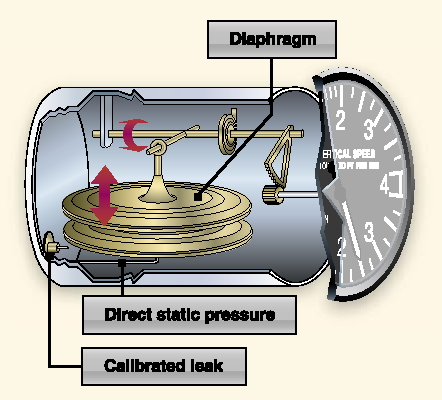
\includegraphics[width=\linewidth]{imagenes/vsi_cropped.pdf}
%   \captionof{Indicador de velocidad vertical}
% \end{minipage}
% \begin{minipage}[b]{0.5\textwidth}
% Constructivamente consta de una carcaza en dónde se recibe el aire del exterior, es decir que el aire se encuentra a la presión externa al avión denominada presión estática. Alrededor de la carcaza hay un fuelle que también se encuentra a la presión exterior, como es evidente ambas son iguales y el instrumento marcara cero, es decir que se vuela nivelado, sin ascenso o descensos.

% En el fuelle se dispone de un tubo capilar calibrado lo que causa un retardo en las variaciones de presión de dicho fuelle, cosa que no ocurre en la carcaza.

% Al ascender o descender la presión sufre variaciones, que son transmitidas inmediatamente a la carcaza, pero por acción del tubo capilar se presentan con retraso en el fuelle, de la comparación entre las dos presiones se obtiene el régimen de ascenso o descenso.
% \end{minipage}

El instrumento tiene también un retardo en la indicación de las variaciones de entre 6 a 9 segundos, además puede presentar oscilaciones en presencia de turbulencias por lo que su precisión y exactitud es muy relativa, debiendo usarse prácticamente para observar tendencias, es decir si los regímenes de ascenso o descenso son crecientes o si se han reducido o incluso estabilizado.


\newpage



\section{Veloc\'imetros. Indicadores de n\'umero de Mach}
\label{sec:Velocimetros.Machmetros}

Los indicadores de velocidad (Velocímetro e Indicador de Número de Mach) forman parte de los sistemas de PITOT-ESTÁTICA de la aeronave, esto es, los que utilizan la información de la presión total y la presión estática que se registra en vuelo por la sonda pitot.

En la Figura \ref{fig:pitot-static.probe} se presenta la forma básica de una sonda pitot-estática donde puede observase la limpieza aerodinámica de las líneas, necesaria para poder efectuarse una medición correcta de las presiones. Una exigencia más, y que no podría cumplirse satisfactoriamente empleando tubos independientes, fue la facilitación de un sistema calefactor par impedir que los tubos se helasen cuando el vuelo se realizase en condiciones de formación de hielo. Los cambios de diseño requeridos dieron lugar a la disposición mostrada en la Figura anteriormente mencionada.

\subsection{Principio de funcionamiento de un veloc\'imetro}
\label{sec:velocimetro.princio.de.funcionamiento}

Los velocímetros son en realidad manómetros muy sensibles que miden las diferencias entre la presión estática y la total detectadas por la sonda pitot, en términos de la siguiente relación:

\begin{equation*}
	p_{\text{\,total}}   - p_{\text{ est\'atica}} = \displaystyle \frac{\rho}{2} \, V^2
\end{equation*}

donde $p_{\text{\,total}} $ representa a la presión total del fluido 
y $p_{\text{ est\'atica}}$ a la estática. 

Despreciando la compresibilidad del aire, se puede despejar de la fórmula anterior la velocidad del mismo:

\begin{equation*}
  \displaystyle
	V = \sqrt{\frac{2 \left(p_{\text{\,total}} -p_{\text{est\'atica}} \right)}{\rho}}
\end{equation*}

la cual se denomina {\bf VELOCIDAD VERDADERA DEL AIRE}, aunque usualmente se la designa por 
{\bf TAS (True Air Speed)}. Como ya es sabido, la densidad del aire, 
$\rho$, varía con la altura de vuelo. 
Por lo tanto sería  necesario sensarla a fin de determinar la TAS.

Para solucionar este inconveniente se utiliza la densidad a nivel del mar calibrada, que se indica en la Tabla de Atmósfera Estandard, la cual tiene el valor de $\rho_0 = 0,001225$\, gr/cm$^3$.

De esta manera, reemplazando en la ecuación de la TAS la densidad correspondiente a la altura de vuelo por la establecida anteriormente se tendrá:

\begin{equation*}
  \displaystyle
	V_e = \sqrt{\frac{2 \left(p_{\text{\,total}} -p_{\text{ est\'atica}} \right)}{\rho_0}}
\end{equation*}

la cual se denomina {\bf VELOCIDAD EQUIVALENTE DEL AIRE}, 
usualmente indicada como {\bf EAS (Equivalent Air Speed)}. 
Este valor sólo corresponde con la TAS a nivel del mar, 
en Atmósfera Estandard y es menor que la TAS a medida que aumenta la altura.

Recordando la diferencia de presiones totales y estáticas en la TAS y EAS, se tiene:

\begin{equation*}
  \begin{array}{lcl}
    p_{\text{\,total}}   - p_{\text{ est\'atica}} = \displaystyle \frac{\rho}{2} \, V^2 & \qquad & \text{TAS} \\
	& & \\
    p_{\text{\,total}}   - p_{\text{ est\'atica}} = \displaystyle \frac{\rho_0}{2} \, Ve^2 & \qquad & \text{EAS} \\
  \end{array}
\end{equation*}

Igualando los segundos miembros queda:

\[
	\displaystyle \frac{\rho}{2} \, V^2
	=
	\displaystyle \frac{\rho_0}{2} \, V_e^2
\]

Despejando la EAS:

\[	\begin{array}{c}
  	V_e^2 = \displaystyle \frac{\rho}{\rho_0}\,V^2 = \sigma \,V^2  \\
	\\
	V_e = \sqrt{\sigma}  V
	\end{array}
\]

Siendo $\sigma = \rho / \rho_0$, la relaci\'on entre las densidades del aire a diferentes
alturas.

Una forma m\'as nemot\'ecnica de recordar lo anterior ser\'ia:

\[\displaystyle
	\text{TAS} = \frac{EAS}{\sqrt{\sigma}}
\]

También se deben tener en cuenta los errores del instrumento debidos a la falta de precisión constructiva del mismo y el error de posición por:

\begin{itemize}
\item Error por distribución de presiones que produce el avión y
  afecta a $p_{\text{ est\'atica}}$
\item Error por actitudes o configuraciones del avión que
  afectan a $p_{\text{\,total}} $.
\end{itemize}

Considerando dichas fallas se obtiene la {\bf VELOCIDAD CALIBRADA DEL AIRE} 
o {\bf CAS (Calibrated Air Speed)}.

Pero tambi\'en deben tenerse en cuenta los efectos de la compresibilidad del aire a grandes velocidades, para lo cual la ecuación de la diferencia de presiones se modifica notablemente mediante la incorporación de nuevos términos. Este efecto se hace más notable a partir de una velocidad de 
250 knots (463 km/hr $\approx 128.61$ m/seg) 
y la ecuación debe reescribirse, considerando que se produce una compresión adiabática en Atmósfera Estandard a nivel del mar.

\begin{equation*}
	p_{\text{\,total}}   - p_{\text{ est\'atica}} = \displaystyle \frac{\rho}{2} \, V_i^2 
	\left( 1 + \frac{1}{4}\,M_0^2
	\right)
\end{equation*}

donde $M_0 = V_i/a_0$, siendo $a_0 \approx 340.25 $ m/seg la  velocidad del sonido a nivel del mar 
y $V_i$ la {\bf VELOCIDAD INDICADA DEL AIRE}  o {\bf IAS (Indicated Air Speed)}. 

De la ecuación anterior, y comparando con la de EAS se deduce: IAS $>$ EAS.

\subsection{Descripción De Un Equipo Típico}
\label{sec:velocimetro.descripcion.equipo.tipico}

El mecanismo del velocímetro que permite transformar la diferencia de presiones en velocidad es una cápsula diferencial que se encuentra conectada a la tubería de presión total mientras que la cámara donde se halla se encuentra sometida a la presión estática. La diferencia de estas presiones provoca la dilatación o contracción de la cápsula, lo cual es transmitido a una aguja indicadora en el panel del instrumento.

\begin{minipage}[b]{0.450\linewidth}
%  \begin{figure}[!h]
    \centering
    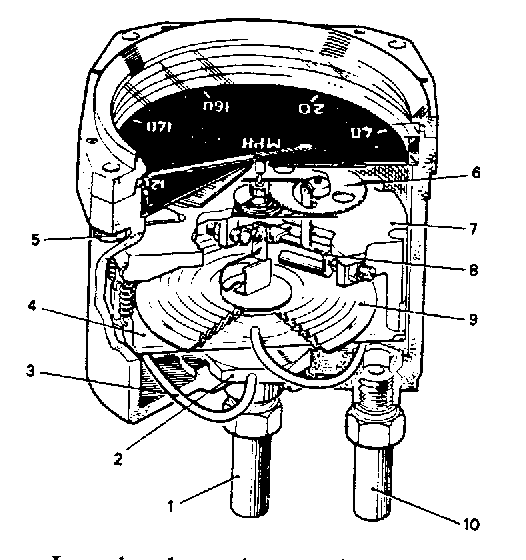
\includegraphics[width=\textwidth]{imagenes/velocimetro.png}
    \captionof{figure}{Disposici\'on interna veloc\'imetro t\'ipico.
	{\footnotesize  1.Tubo de presión total. 2.Niple. 3.Capilar. 4.Placa base. 5.Tornillo de  sujeción. 6.Brazo del sector. 7.Soporte superior. 8.Eje rotante. 9.Cápsula diferencial. 10. Tubo de presión estática.}
}
    \label{fig:velocimetro.tipico}
%  \end{figure}
\end{minipage}
\hspace{0.0250\linewidth}
\begin{minipage}[b]{0.50\linewidth}
  En la Figura \ref{fig:velocimetro.tipico} puede apreciarse la construcción de un velocímetro
  típico.

  El conjunto resulta muy compacto y con mecanismos de precisión. Los
  desplazamientos de la cápsula siguen lo que se denomina \textbf{Ley
    Cuadr\'atica} debido a la transmisión de las dilataciones o
  contracciones de la cápsula a través del sistema mecánico. La
  compensación de temperatura se logra mediante una tira bimetálica
  dispuesta para que la multiplicación del sistema de palanca varíe en
  oposición a los efectos de la temperatura en la sensibilidad de la
  cápsula y el sistema.

Puesto que los velocímetros miden una diferencia de presión que varía con el cuadrado de la velocidad, ocurre que si las deflexiones de la cápsulas respondiesen linealmente a la presión, la respuesta característica del sistema con respecto a la velocidad sería análoga a la que se muestra en la Figura \ref{fig:ley.cuadratica}.

 Si la cápsula también estuviese acoplada al mecanismo de la aguja de forma que sus deflexiones fuesen aumentadas directamente, la escala del instrumento sería la del tipo indicado en la Figura \ref{fig:ley.cuadratica}.

\end{minipage}

\begin{figure}[!h]
  \centering
  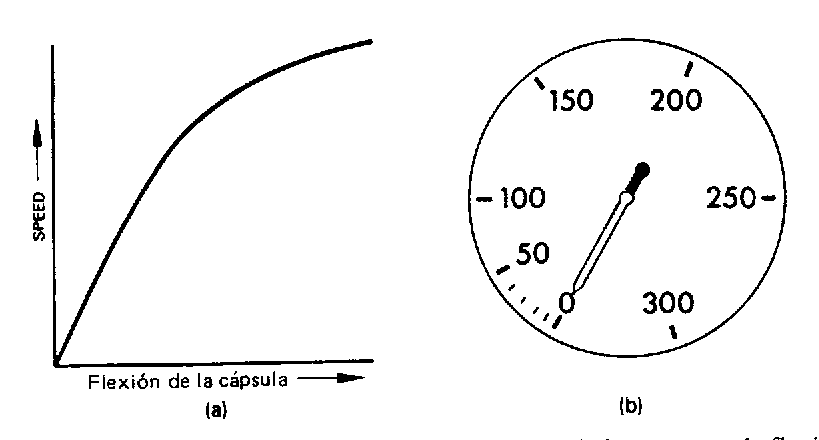
\includegraphics[width=0.9\textwidth]{imagenes/velocimetro_ley_cuadratica.png}
  \caption{Ley cuadr\'atica}
  \label{fig:ley.cuadratica}
\end{figure}


La no linealidad de tal escala hace que sea difícil de leer con exactitud, particularmente en el extremo bajo de la gama de velocidad; además la longitud de la escala para una gama amplia de velocidad sería demasiado grande para los tamaños estandard de cajas.

Por consiguiente, para obtener la linealidad deseada se necesita un método para controlar la característica de la cápsula o la dimensión del elemento de acoplamiento que las flexiones de la cápsula transmiten a la aguja. De los dos métodos, el más prácti




\newpage

\section{Computadores centrales de datos de aire}
\label{sec:Computadores.centrales.de.datos.de.aire}

Los Computadores Centrales de Datos de Aire o, simplemente, Computadores de Datos de Aire
 (ADC = Air Data Computer) 

Las presiones y temperaturas se reciben en un lugar centralizado de la aeronave, son medidas, comparadas,
corregidas para subsanar errores de diferente naturaleza y se utiliza esta informaci\'on
para realizar c\'alculos.
Los resultados son enviados electr\'onicamente a diferentes indicadores.

Central Air Data Computer (CADC) 
entre 1968 y 1970 la primer CADC digital se produjo para el caza F-14A Tomcat.

Existen multitud de sistemas de datos del aire distintos según el fabricante, por ejemplo, en
Airbus los ADC (air data computer) se combinan con los sistemas de altitud, rumbo, y
navegaci\'on del tipo IRS para formar un sistema denominado Air Data Inertial Reference
Unit o (ADIRU). En los modernos aparatos que salen de la factorías de BOEING y AIRBUS se
están reemplazando por lo más modernos sistemas denominados Global Navigation Air Data
Inertial Reference System (GNADIRS). Estos sistemas son modelos muy avanzados que
integran normalmente tres subsistemas esenciales que antes se encontraban separados. Estos
sistemas son el GPS (o GNSS), el IRS y el ADC.

La tendencia en sistemas de avi\'onica es la de
tener todos esto sistemas juntos para ofrecer una mejor integraci\'on, menor peso y mayor
eficiencia energética. En aviones modernos como el Boeing 777, estos sistemas son tarjetas
electr\'onicas  que forman parte de una carcasa y que se
pueden cambiar en linea de vuelo en caso de avería. Son las denominadas ``Plug and Fly'' en
consonancia con las de los PC's ``Plug and play'' (conectar y listo). La misi\'on fundamental de la
placa dedicada al GPS/GNSS es la de proveer datos precisos de posici\'on, altitud geométrica, y
velocidad sobre el suelo al sistema de gesti\'on de vuelo FMS o Flight Management system (a
veces llamado FMGS - Flight Management and Guidance System).



\newpage

\bibliographystyle{plain}
\bibliography{../IyA}
%\bibliographystyle{plain}
%\bibliography{sample}

%Gracey, William (1980), ``Measurement of Aircraft Speed and Altitude'', NASA Reference Publication 1046. \url{http://www.dtic.mil/dtic/tr/fulltext/u2/a280006.pdf}



\end{document}




%
%  Asi se citan las direcciones web
%
%Example usage
%
%In the preamble:
%---------------
%
%\usepackage{url}
%
%% Define a new 'leo' style for the package that will use a smaller font.
%\makeatletter
%\def\url@leostyle{
%  \@ifundefined{selectfont}{\def\UrlFont{\sf}}{\def\UrlFont{\small\ttfamily}}}
%\makeatother
%
% Now actually use the newly defined style.
%
%\urlstyle{leo}
%
%
%In a BibTeX entry:
%------------------
%
%@misc{
%    c.elmohamed,
%    author = "Saleh Elmohamed",
%    title = "Examples in {H}igh {P}erformance {F}ortran",
%    howpublished = "Website",
%    year = {1996},
%    note = {\url{http://www.npac.syr.edu/projects/
%                    cpsedu/summer98summary/ examples/hpf/hpf.html}}
%}




